\section{Results}
-- describe pro-time vs pro-route scenarios
-- describe battery capacities
-- describe maximum charge rates
-- describe how route scheduels, delta, and uncontrolled loads come from uta.
-- describe the gaps used in the minimisation algorithms.
\subsection{Comparison with Prior Work}
In this section, we compare the proposed method with a baseline algorithm and a method developed be \textcolor{red}{insert reference to He. et al here}. The baseline method models how bus drivers charge their electric vehicles at the Utah Transit Authority in Salt Lake City, Utah. At UTA, when bus drivers arrive at the station, they refuel their electric buses whenever a charger is available so that the number of charge sessions is maximized. The method from \textcolor{red}{He et al.} works somewhat differently by minimising the cost of energy with respect to the time of use tarrifs $\mu_{e-on}$ and $\mu_{e-off}$.
\par The comparison we observe is given for a 5-bus, 5-charger scenario with a pro-time preference and a single group. Each method was run, and the cost related to demand, facilities, and energy charges are given in Fig. \ref{fig:results:costComparison}. Note how the baseline algorithm suffers significantly from the demand charges associated with On-Peak Power, and \textcolor{red}{He et al.} incurres additional cost from the facilities charges, indicating that an emphasis on energy charges and habitual charging patterns can be improved.
\par We observe where the differences in cost originate in Fig. \ref{fig:results:totalPower}. Observe how the baseline charge profile achieved the largest 15-minute average power between 19:12 adn 21:36 which is during on-peak hours and consequently yielded the large On-Peak Power charges given in Fig. \ref{fig:results:costComparison}. Additionally, note how the proposed method maintains a relatively flat power profile so that the load is balanced throughout the day which we investigate in Fig. \ref{fig:results:powerPlot}.
\par We investigate how t 
\begin{figure}
	\centering
	\makeComparisonBarChartThree{media/11_results/costComparison.csv}{Cost (Dollars)}{Baseline}{He et al.}{Proposed}
	\caption{Cost comparison with prior work}
	\label{fig:results:costComparison}
\end{figure} 

 
\begin{figure*}
	\centering
	\makeComparisonPower{media/11_results/powerPlotfiscal.csv}{media/11_results/powerPlotconsumption.csv}{15-Minute Average Power (kW)}{Proposed}{He et al.}
	\caption{Comparison between uncontrolled and bus loads}
	\label{fig:results:powerPlot}
\end{figure*}


\begin{figure*}
	\centering
	\makeComparisonTotalPower{media/11_results/totalPowerfiscalproTime.csv}{media/11_results/totalPowerconsumptionproTime.csv}{15-Minute Average Power (kW)}{Proposed}{He et al.}
	\caption{15-Minute average power for one day}
	\label{fig:results:totalPower}
\end{figure*}



\subsection{Contention: Sub-Optimal Schedules}
show comparison of schedules with large vs small gaps when finding charge schedules. Talk about how the computation time significantly increases as the gap decreases. Show that a smaller gap may be desireable as this lengthens charge times so that they are easier to implement in reality. Explain that we trade time for longer charge sessions better suited for operations.
\input{media/11_results/disoptimalRoutes.tex}
\input{media/11_results/sessionImageStyle}
\begin{figure*}
\begin{tikzpicture}
\begin{axis}[colorbar, ChargeSessionImage, width=0.95\textwidth, height=0.5\textwidth, point meta min=0, point meta max=350, xmin=0.5, xmax=4320.5,xtick={540, 1080, 1620, 2160, 2700, 3240, 3780, 4320}, xticklabels={3:00, 6:00, 9:00, 12:00, 15:00, 18:00, 21:00, 0:00}, ymin=0.5, ymax=18.5]

\addplot [forget plot] graphics [xmin=0.5, xmax=4320.5, ymin=0.5, ymax=18.5] {media/11_results/optimalRoutes-1.png};
\end{axis}

\end{tikzpicture}%
\caption{Routes with a small gap in the route placement problem}
\label{fig:results:optimalRoutes}
\end{figure*}


\subsection{Contested vs Uncontested}
address that there is significantly more computations for the schedules that are operations-oriented, and use this to segway into groups
\begin{figure}
	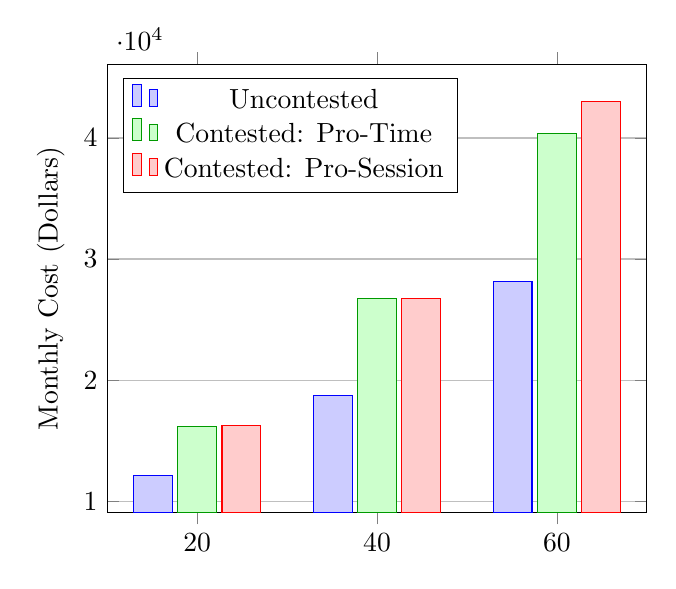
\begin{tikzpicture}
		\begin{axis}[ybar, bar width=14pt, xmin=10, xmax=70, xtick={20, 40, 60},ymajorgrids=true, ylabel={Monthly Cost (Dollars)}, legend pos=north west]
			\addplot[fill=blue!20, draw=blue] coordinates {
				(20, 12150.65)
				(40, 18745.58)
				(60, 28166.09)
			};
			\addplot[fill=green!20, draw=black!40!green] coordinates {
				(20, 16183.79)
				(40, 26738.71)
				(60, 40405.72)
			};
			\addplot[fill=red!20, draw=red] coordinates {
				(20, 16256.21)
				(40, 26738.71)
				(60, 43007.78)
			};
		\legend{Uncontested, Contested: Pro-Time, Contested: Pro-Session};
		\end{axis}
	\end{tikzpicture}
	\caption{Comparison of Monthly Costs}
	\label{fig:results:contestedVsUncontestedPrice}
\end{figure}



\begin{figure}\centering
	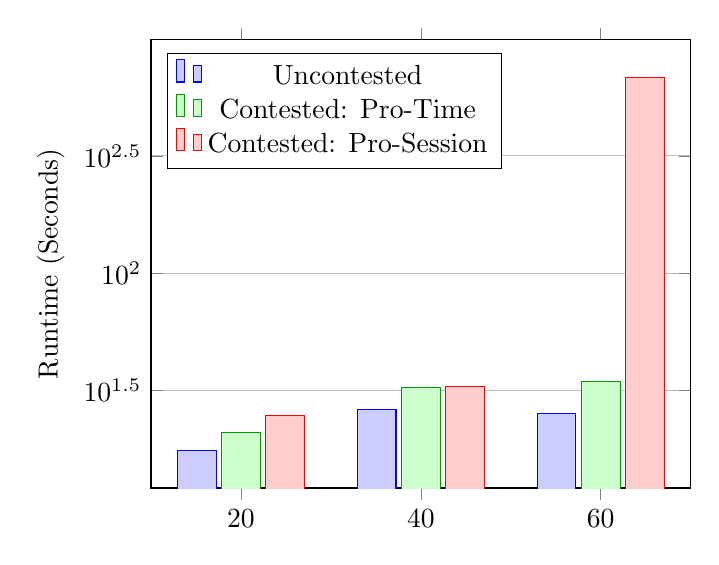
\begin{tikzpicture}
		\begin{axis}[ybar, bar width=14pt, xmin=10, xmax=70, xtick={20, 40, 60},ymajorgrids=true, ylabel={Runtime (Seconds)}, ymode=log, legend pos=north west]
			\addplot[fill=blue!20, draw=blue] coordinates {
				(20, 17.46)
				(40, 26.09)
				(60, 25.17)
			};
			\addplot[fill=green!20, draw=black!40!green] coordinates {
				(20, 20.84)
				(40, 32.47)
				(60, 34.46)
			};
			\addplot[fill=red!20, draw=red] coordinates {
				(20, 24.57)
				(40, 32.70)
				(60, 686.40)
			};
		\legend{Uncontested, Contested: Pro-Time, Contested: Pro-Session};
		\end{axis}
	\end{tikzpicture}
	\caption{Comparison of Runtimes} 
	\label{fig:results:contestedVsUncontestedTime}
\end{figure}



%\begin{figure}
	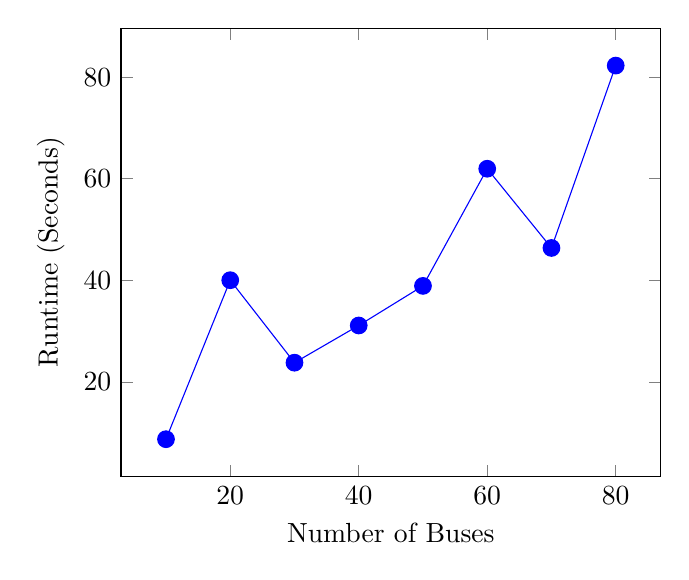
\begin{tikzpicture}
		\begin{axis}[xlabel=Number of Buses,  ylabel=Runtime (Seconds)]
			\addplot[blue] coordinates {
				(10, 8.69)
				(20, 40.01)
				(30, 23.76)
				(40, 31.09)
				(50, 38.89)
				(60, 61.97)
			  (70, 46.36 )
			  (80, 82.29)};
			\addplot[blue, only marks, mark size=3pt] coordinates {
			  (10, 8.69)
				(20, 40.01)
				(30, 23.76)
				(40, 31.09)
				(50, 38.89)
				(60, 61.97)
			  (70, 46.36 )
			  (80, 82.29)};
		\end{axis}
	\end{tikzpicture}
	\caption{Uncontested Runtime} 
	\label{fig:uncontestedRuntime}
\end{figure}



%\begin{figure}
	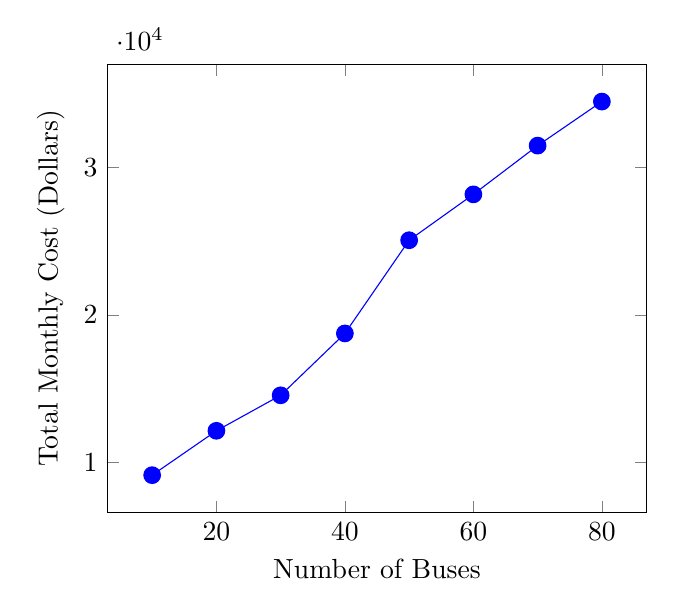
\begin{tikzpicture}
		\begin{axis}[xlabel=Number of Buses, ylabel=Total Monthly Cost (Dollars), legend pos=north west, legend style={nodes={scale=0.7}}]
			\addplot[blue] coordinates {
				(10,  9145.28)
				(20, 12150.65)
				(30, 14554.62)
				(40, 18745.58)
				(50, 25059.45)
				(60, 28166.09)
				(70, 31468.65)
				(80, 34452.85)}; 
			\addplot[blue, only marks, mark size=3pt] coordinates {
				(10,  9145.28)
				(20, 12150.65)
				(30, 14554.62)
				(40, 18745.58)
				(50, 25059.45)
				(60, 28166.09)
				(70, 31468.65)
				(80, 34452.85)}; 
			%\legend{Proposed, Baseline, He et al.}
		\end{axis}
	\end{tikzpicture}
	\caption{Monthly Cost With Contention with emphasis on time}
	\label{fig:scalabilityCostContentionProTime}
\end{figure}



%\begin{figure}
	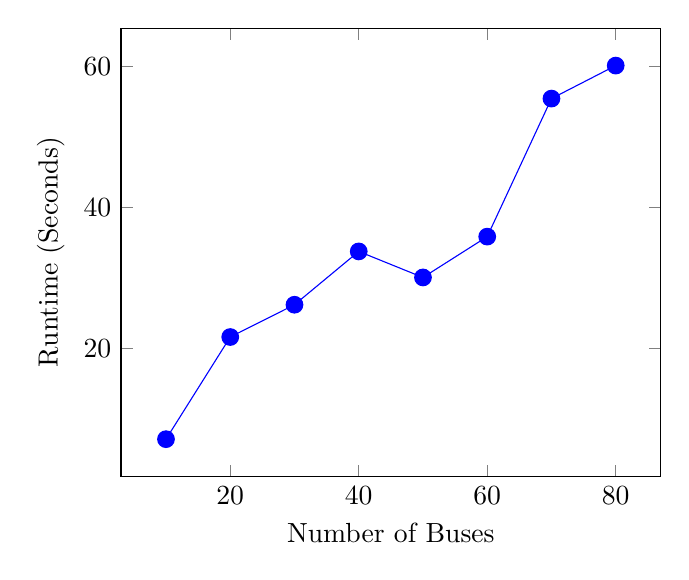
\begin{tikzpicture}
		\begin{axis}[xlabel=Number of Buses,  ylabel=Runtime (Seconds)]
			\addplot[blue] coordinates {
				(10, 7.15)
				(20, 21.64)
				(30, 26.22)
				(40, 33.78)
				(50, 30.09)
				(60, 35.88)
			  (70, 55.46 )
			  (80, 60.14)};
			\addplot[blue, only marks, mark size=3pt] coordinates {
				(10, 7.15)
				(20, 21.64)
				(30, 26.22)
				(40, 33.78)
				(50, 30.09)
				(60, 35.88)
			  (70, 55.46 )
			  (80, 60.14)};
		\end{axis}
	\end{tikzpicture}
	\caption{Runtime with contention with time prioritized} 
	\label{fig:uncontestedRuntime}
\end{figure}




\subsection{Contention: The Importance of Groups}
Show time difference between 1, 2, and 3 groups when optimizing for cost, talk about how this disparity significantly increases as the gap requirements decrease.
\begin{figure}
\centering
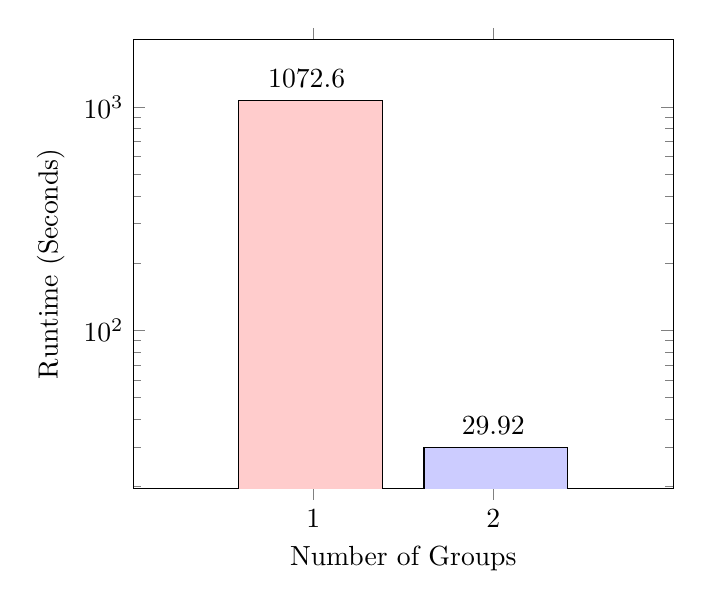
\begin{tikzpicture}
	\begin{axis}[ybar, ymode=log, ymax=2000, xmin=0, xmax=3, xtick={1,2}, xlabel=Number of Groups, ylabel=Runtime (Seconds)]
		\addplot[fill=red!20, bar width=0.8] coordinates {(1.4, 1072.6)};
		\addplot[fill=blue!20, bar width=0.8]  coordinates {(1.6, 29.92)};
	\end{axis}
	\node at (2.2,5.2){1072.6};
	\node at (4.57, 0.79){29.92};
\end{tikzpicture}
\caption{Runtimes for a 18 bus 12 charger scenario at a 0.13\% gap}
\label{fig:results:groupResults}
\end{figure}

\subsection{Effecrts of De-Fragmentation}
display heat map of before and after for contested case.
\begin{figure*}
\centering
\begin{tikzpicture} 
\begin{axis}[colorbar, ChargeSessionImage, width=5.2in, height=2in, point meta min=0, point meta max=350, xmin=0.5, xmax=4320.5, xtick={540, 1080, 1620, 2160, 2700, 3240, 3780, 4320}, xticklabels={3:00, 6:00, 9:00, 12:00, 15:00, 18:00, 21:00, 0:00}, ymin=0.5, ymax=40.5]
\addplot [forget plot] graphics [xmin=0.5, xmax=4320.5, ymin=0.5, ymax=40.5] {\rootdirectorythree/media/11_results/defragmentedChargeLimit-1.png}; 
\end{axis} 
\end{tikzpicture}
\caption{Routes with De-Fragmentation}
\label{fig:results:defragmentedChargeLimit}
\end{figure*}

\begin{figure*}
\centering
\begin{tikzpicture} 
\begin{axis}[colorbar, ChargeSessionImage, width=0.95\textwidth, height=0.5\textwidth, point meta min=0, point meta max=350, xmin=0.5, xmax=4320.5, xtick={540, 1080, 1620, 2160, 2700, 3240, 3780, 4320}, xticklabels={3:00, 6:00, 9:00, 12:00, 15:00, 18:00, 21:00, 0:00}, ymin=0.5, ymax=40.5]
\addplot [forget plot] graphics [xmin=0.5, xmax=4320.5, ymin=0.5, ymax=40.5] {media/11_results/noFragmentationChargeLimit-1.png}; 
\end{axis} 
\end{tikzpicture}
\caption{Routes without De-Fragmentation}
\label{fig:results:noFragmentationChargeLimit}
\end{figure*}


describe how defragmentation affects runtime and cost in the case of time-oriented and operations-oriented approaches.
\begin{figure}\centering
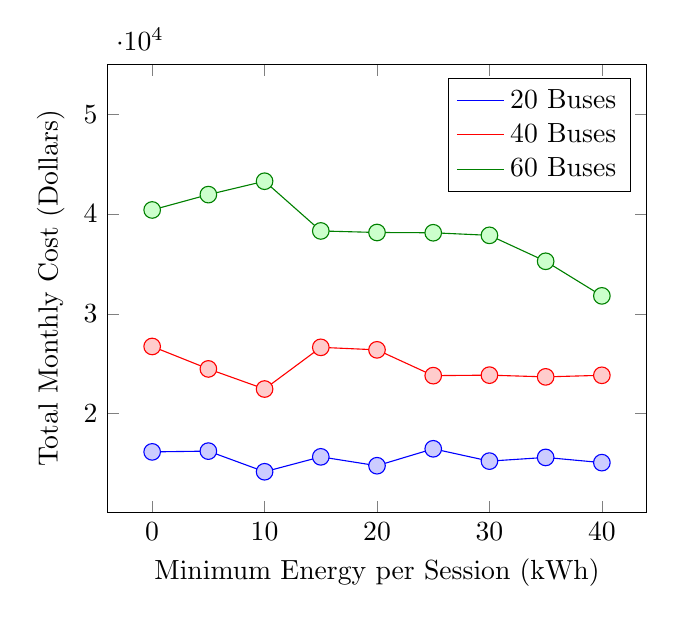
\begin{tikzpicture}
\begin{axis}[xlabel=Minimum Energy per Session (kWh), ylabel=Total Monthly Cost (Dollars), ymax=55000, legend pos=north east]
	\addplot[blue] coordinates {
		(0, 16183.79)   
	  (5, 16260.98)  
		(10,14194.10)  
		(15,15686.16)  
		(20,14798.53)  
		(25,16492.56)  
		(30,15259.19)  
		(35,15628.38)  
		(40,15106.82)};
\addplot[red] coordinates {
		(0, 26738.71)
		(5, 24491.03)
	  (10,22476.88)
		(15,26650.71)
		(20,26400.31)
		(25,23816.91)
		(30,23866.55)
		(35,23693.25)
		(40,23851.78)};
\addplot[green!50!black] coordinates {
		(0, 40405.72)
		(5, 41942.45)
	  (10,43284.09)
		(15,38304.96)
		(20,38150.28)
		(25,38122.51)
		(30,37864.79)
		(35,35268.11)
		(40,31805.12)};

\addplot[blue!20, draw=blue, only marks, mark size=3pt] coordinates {
		(0, 16183.79)  
		(5, 16260.98)  
	  (10,14194.10)  
		(15,15686.16)  
		(20,14798.53)  
		(25,16492.56)  
		(30,15259.19)  
		(35,15628.38)   
		(40,15106.82)};
\addplot[red!20, draw=red, only marks, mark size=3pt] coordinates {
	(0, 26738.71)  	
	(5, 24491.03)  	
	(10,22476.88)   
	(15,26650.71)  	
	(20,26400.31)  	
	(25,23816.91)  	
	(30,23866.55)  	
	(35,23693.25)  	
	(40,23851.78)};	
\addplot[green!20, draw=green!50!black, only marks, mark size=3pt] coordinates {
	(0, 40405.72)  
	(5, 41942.45)  
	(10,43284.09)  
	(15,38304.96)  
	(20,38150.28)  
	(25,38122.51)  
	(30,37864.79)  
	(35,35268.11)  
	(40,31805.12)};

\legend{20 Buses, 40 Buses, 60 Buses} 
\end{axis}
\end{tikzpicture}
\caption{Cost comparison of different degragmentation thresholds in a pro-time optimization scheme.}
\label{fig:results:defragmentationCostProTime}
\end{figure}

\begin{figure}
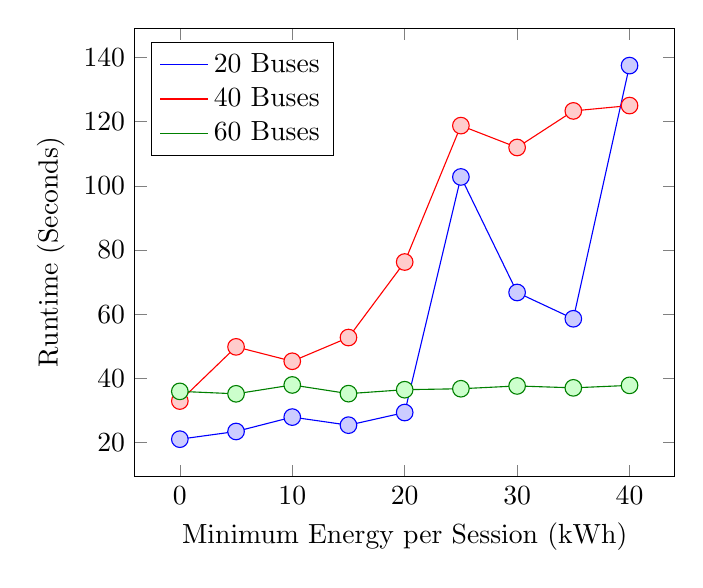
\begin{tikzpicture}
\begin{axis}[xlabel=Minimum Energy per Session (kWh), ylabel=Runtime (Seconds), legend pos=north west]
	\addplot[blue] coordinates {
		(0, 21.00)
		(5, 23.40)
	  (10,27.89)
		(15,25.37)
		(20,29.31)
		(25,102.78)
		(30,66.75)
		(35,58.55)
		(40,137.51)}; 
\addplot[red] coordinates {
		(0, 32.89)
		(5, 49.79)
	  (10,45.30)
		(15,52.70)
		(20,76.25)
		(25,118.79)
		(30,111.97)
		(35,123.37)
		(40,125.04)}; 
\addplot[green!50!black] coordinates {
		(0, 35.91)
		(5, 35.15)
	  (10,37.91)
		(15,35.20)
		(20,36.43)
		(25,36.73)
		(30,37.60)
		(35,37.01)
		(40,37.78)}; 
\addplot[blue!20, draw=blue, only marks, mark size=3pt] coordinates {
		(0, 21.00)
		(5, 23.40)
	  (10,27.89)
		(15,25.37)
		(20,29.31)
		(25,102.78)
		(30,66.75)
		(35,58.55)
		(40,137.51)}; 
\addplot[red!20, draw=red, only marks, mark size=3pt] coordinates {
		(0, 32.89)
		(5, 49.79)
	  (10,45.30)
		(15,52.70)
		(20,76.25)
		(25,118.79)
		(30,111.97)
		(35,123.37)
		(40,125.04)}; 
\addplot[green!20, draw=green!50!black, only marks, mark size=3pt] coordinates {
		(0, 35.91)
		(5, 35.15)
	  (10,37.91)
		(15,35.20)
		(20,36.43)
		(25,36.73)
		(30,37.60)
		(35,37.01)
		(40,37.78)}; 
\legend{20 Buses, 40 Buses, 60 Buses}		
\end{axis}
\end{tikzpicture}
\caption{Comparison of runtime for the uncontested and contested scenarios over different de-fragmentation criteria}
\label{fig:results:runtimeDefragmentation}
\end{figure}

\begin{figure}
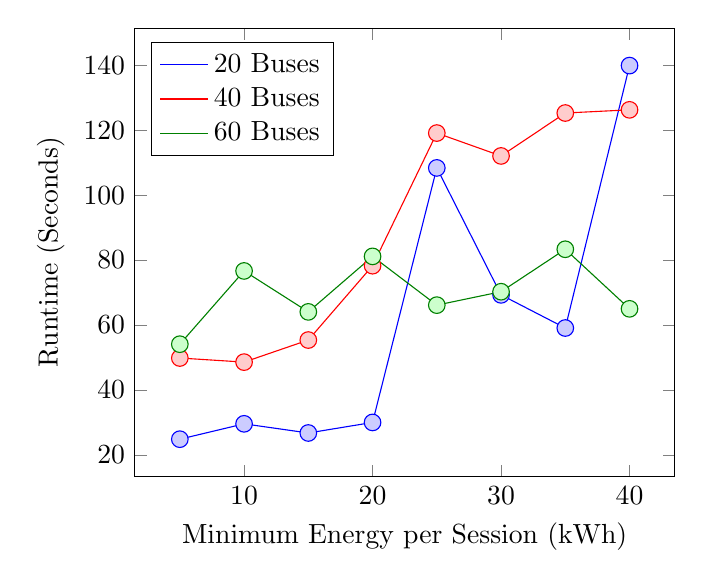
\begin{tikzpicture}
\begin{axis}[xlabel=Minimum Energy per Session (kWh), ylabel=Runtime (Seconds), legend pos=north west]
	\addplot[blue] coordinates {
		(5, 24.83)
	  (10,29.56)
		(15,26.74)
		(20,29.99)
		(25,108.38)
		(30,69.28)
		(35,59.07)
		(40,139.90)}; 
\addplot[red] coordinates {
		(5, 49.83)
	  (10,48.57)
		(15,55.37)
		(20,78.26)
		(25,119.12)
		(30,112.07)
		(35,125.29)
		(40,126.27)}; 
\addplot[green!50!black] coordinates {
		(5, 54.09)
	  (10,76.65)
		(15,64.04)
		(20,81.13)
		(25,66.12)
		(30,70.25)
		(35,83.33)
		(40,64.98)}; 
\addplot[blue!20, draw=blue, only marks, mark size=3pt] coordinates {
		(5, 24.83)
	  (10,29.56)
		(15,26.74)
		(20,29.99)
		(25,108.38)
		(30,69.28)
		(35,59.07)
		(40,139.90)}; 
\addplot[red!20, draw=red, only marks, mark size=3pt] coordinates {
		(5, 49.83)
	  (10,48.57)
		(15,55.37)
		(20,78.26)
		(25,119.12)
		(30,112.07)
		(35,125.29)
		(40,126.27)}; 
\addplot[green!20, draw=green!50!black, only marks, mark size=3pt] coordinates {
		(5, 54.09)
	  (10,76.65)
		(15,64.04)
		(20,81.13)
		(25,66.12)
		(30,70.25)
		(35,83.33)
		(40,64.98)}; 
\legend{20 Buses, 40 Buses, 60 Buses}		
\end{axis}
\end{tikzpicture}
\caption{Comparison of runtimes for various defragmentation scenarios in a pro-session environment}
\label{fig:results:defragmentationTimeProSchedule}
\end{figure}

\begin{figure}
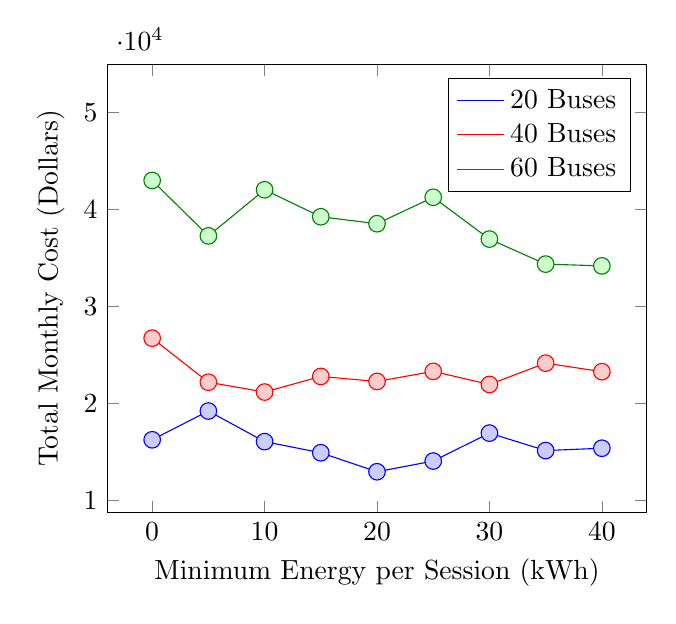
\begin{tikzpicture}
\begin{axis}[xlabel=Minimum Energy per Session (kWh), ylabel=Total Monthly Cost (Dollars), ymax=55000, legend pos=north east]
	\addplot[blue] coordinates {
		(0, 16256.21)   
	  (5, 19221.75)  
		(10,16068.21)  
		(15,14919.20)  
		(20,12958.06)  
		(25,14062.05)  
		(30,16946.17)  
		(35,15143.95)  
		(40,15386.03)};
\addplot[red] coordinates {
		(0, 26738.71)
		(5, 22196.87) 
	  (10,21180.43)
		(15,22789.78)
		(20,22273.05)
		(25,23312.12)
		(30,21963.29)
		(35,24164.56)
		(40,23282.00)};
\addplot[green!50!black] coordinates {
		(0, 43007.78)
		(5, 37289.58)
	  (10,42044.81)
		(15,39261.70)
		(20,38546.15)
		(25,41271.99)
		(30,36959.39)
		(35,34377.97)
		(40,34195.29)}; 
\addplot[blue!20, draw=blue, only marks, mark size=3pt] coordinates {
		(0, 16256.21)   
	  (5, 19221.75)  
		(10,16068.21)  
		(15,14919.20)  
		(20,12958.06)  
		(25,14062.05)  
		(30,16946.17)  
		(35,15143.95)  
		(40,15386.03)};
\addplot[red!20, draw=red, only marks, mark size=3pt] coordinates {
		(0, 26738.71)
		(5, 22196.87) 
	  (10,21180.43)
		(15,22789.78)
		(20,22273.05)
		(25,23312.12)
		(30,21963.29)
		(35,24164.56)
		(40,23282.00)};
\addplot[green!20, draw=green!50!black, only marks, mark size=3pt] coordinates {
		(0, 43007.78)
		(5, 37289.58)
	  (10,42044.81)
		(15,39261.70)
		(20,38546.15)
		(25,41271.99)
		(30,36959.39)
		(35,34377.97)
		(40,34195.29)}; 
\legend{20 Buses, 40 Buses, 60 Buses} 
\end{axis}
\end{tikzpicture}
\caption{Cost comparison of different degragmentation thresholds in a pro-schedule optimization scheme.}
\label{fig:results:costDefragmentationProTime}
\end{figure}


	
	
